% ============================================================================
% CURRICULUM VITAE
%
% BU guide 1.9: required of ALL doctoral and master's candidates, and it must be
% the LAST numbered page(s) of the document. Aim for three or four pages.
% Required content: your full name and a contact address (your department is
% fine) where you can be reached for the next one to two years.
%
% ---------------------------------------------------------------------------
% SOURCE: ~/Desktop/resume-2025/resume  (the standalone resume LaTeX project)
%
% This page is NOT edited here. To change it, edit the resume project, then:
%
%     bash document/cv/build-cv.sh      # regenerates graphics/cv.pdf
%     bash document/build.sh            # rebuilds the dissertation
%
% build-cv.sh re-typesets the resume at BU margins (top 1.5in, left 1.5in,
% right 1in) via document/cv/cv-bu.tex. It deliberately re-typesets rather than
% scaling the resume's own PDF, because scaling would push the 11pt body text
% below the 10pt minimum in BU guide 1.1.2.
% ---------------------------------------------------------------------------

\newpage
\phantomsection%
\addcontentsline{toc}{chapter}{Curriculum \texorpdfstring{Vit\ae}{Vitae}}

% pagecommand puts the dissertation's own running page number on each included
% page -- the resume project sets \pagestyle{empty}, and BU guide 1.1.4
% requires every page through the last page of the vita to be numbered.
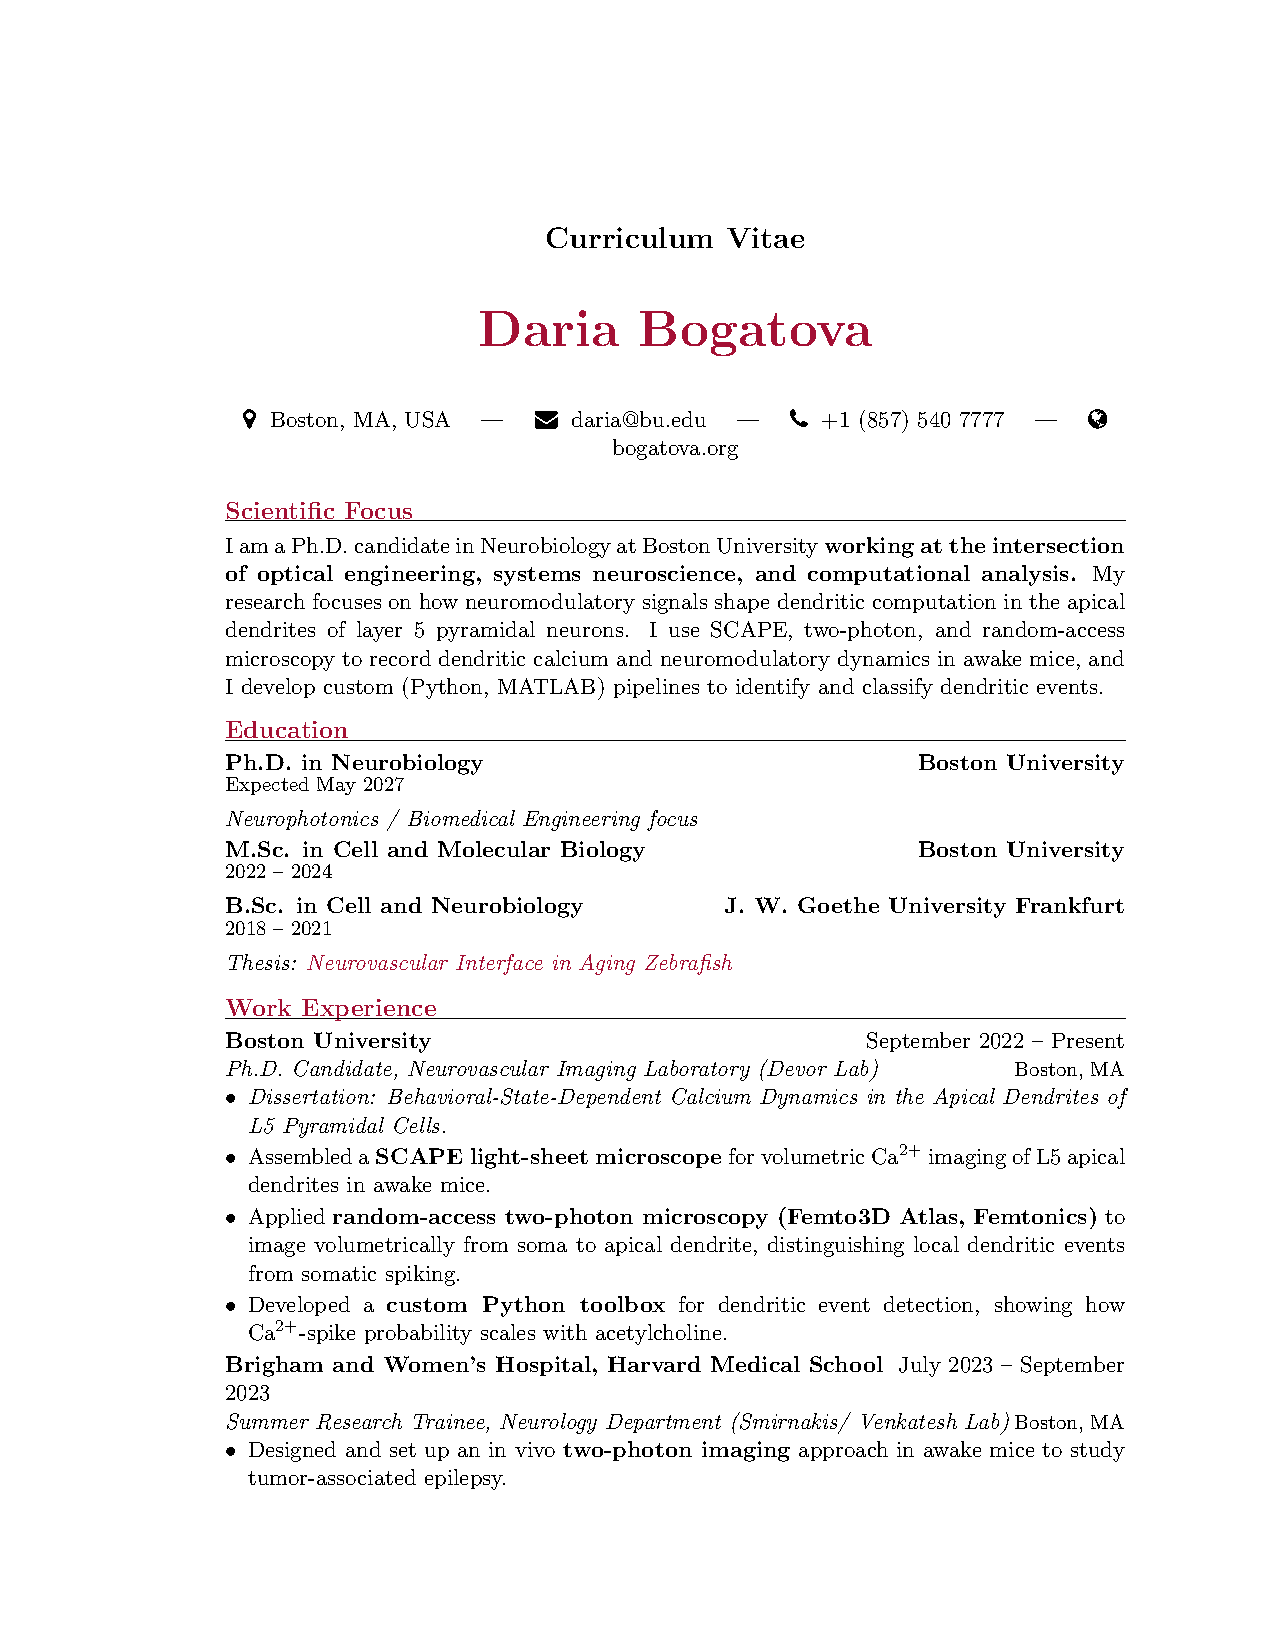
\includepdf[
	pages         = -,
	pagecommand   = {\thispagestyle{myheadings}},
	fitpaper      = false,
	offset        = 0 0
]{graphics/cv.pdf}
